%!TEX TS-program = xelatex
\documentclass{beamer}

\usepackage{HSE-theme/beamerthemeHSE-en} % Load HSE theme

%%% Fonts 
\usepackage{fontspec}
%\defaultfontfeatures{Ligatures={TeX},Renderer=Basic}
%\setmainfont[Ligatures={TeX,Historic}]{Myriad Pro} % install Myriad Pro or replace with Arial
%\setsansfont{Myriad Pro}  % install Myriad Pro or replace with Arial
%\setmonofont{Courier New}
\newcommand*{\Scale}[2][4]{\scalebox{#1}{$#2$}}%
\newcommand*{\Resize}[2]{\resizebox{#1}{!}{$#2$}}%
\usepackage{multicol} 		% Multiple columns
\graphicspath{{Images/}}  	% Images folder

 


%%% Author and speech
\title[Short title]{Globule-coil Transition in Models of Linear Magnetic Polymers} 
%\subtitle{Presentation Subtitle or Conference Title}
\author[ ]{Kamilla Faizullina \\ \smallskip \scriptsize \url{knfayzullina@edu.hse.ru}\\\url{  }}
%\institute[Higher School of Economics]{National Research University \\ Higher School of Economics (Moscow)}
\institute[Higher School of Economics]{Supervisor: Evgeni Burovski}
\date{01.06.2022} 
\begin{document}	% Document begins

\frame[plain]{\titlepage}	% Title frame

\section{Just some text}
\subsection{Subtitle}

\begin{frame}
\frametitle{XY model on self-avoiding walks (SAWs)}
 	\begin{multicols}{2}
  
 		\begin{itemize}
 			\item Magnetic polymer is a sequence of $N$ monomers 
 			\item Conformation is a self-avoiding walk
 			\item Each node represents a spin-like variable $s_i$ associated with angle $\theta_i \in  [-\pi;\pi]$
 		\end{itemize}
   
 	\columnbreak
  
   \begin{figure}[H]
  	\centering
  	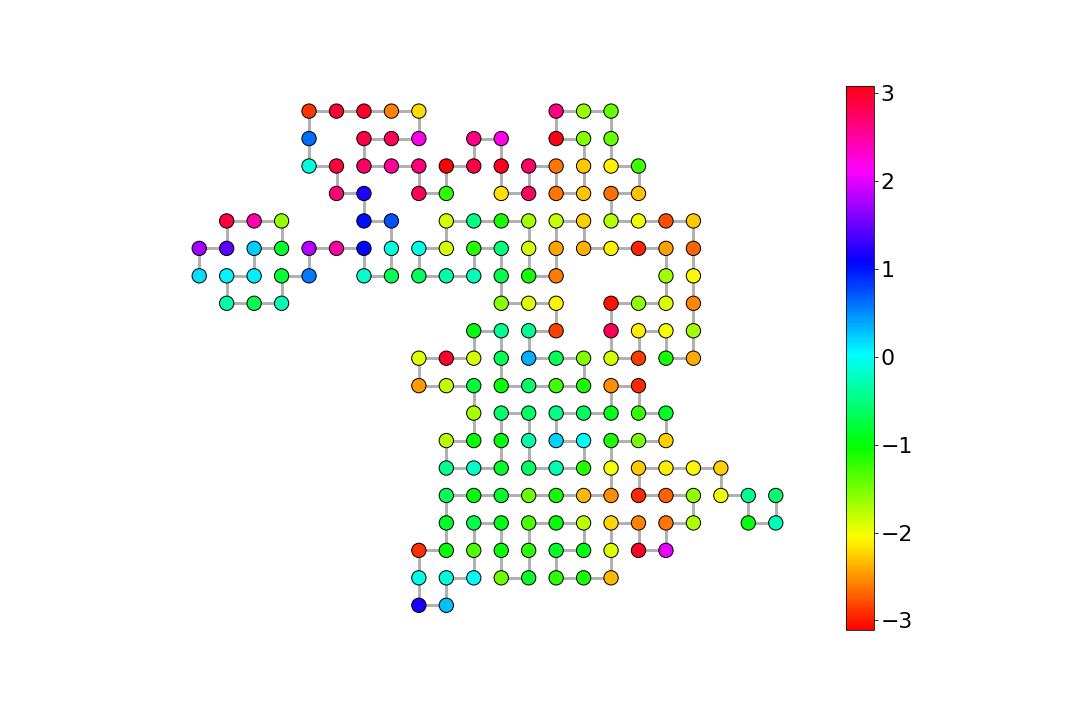
\includegraphics[scale=0.13]{state_example2.png} \\ 
  	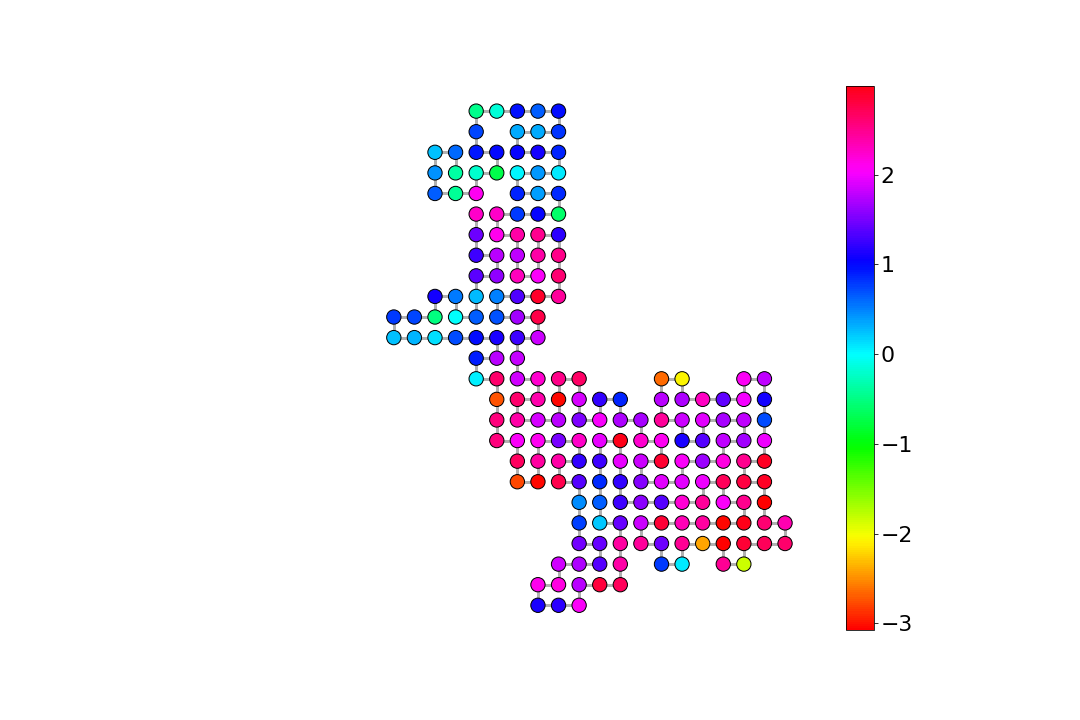
\includegraphics[scale=0.13]{state_example1.png}
  	%\caption{   }
  	\label{fig:example}
  \end{figure}
  
 \end{multicols}
\end{frame}



\begin{frame}
	\frametitle{XY model on self-avoiding walks (SAWs)}
	\begin{multicols}{2}
		
		\begin{itemize}
			\item Hamiltonian in lack of an external field: 
			\begin{equation*}
			H(u,s) = -J \sum_{ \langle i, j \rangle } cos(\theta_i - \theta_j)  
			\end{equation*}
			%\item 
			
			
		\end{itemize}
		
		\columnbreak
		
		\begin{figure}[H]
			\centering
  	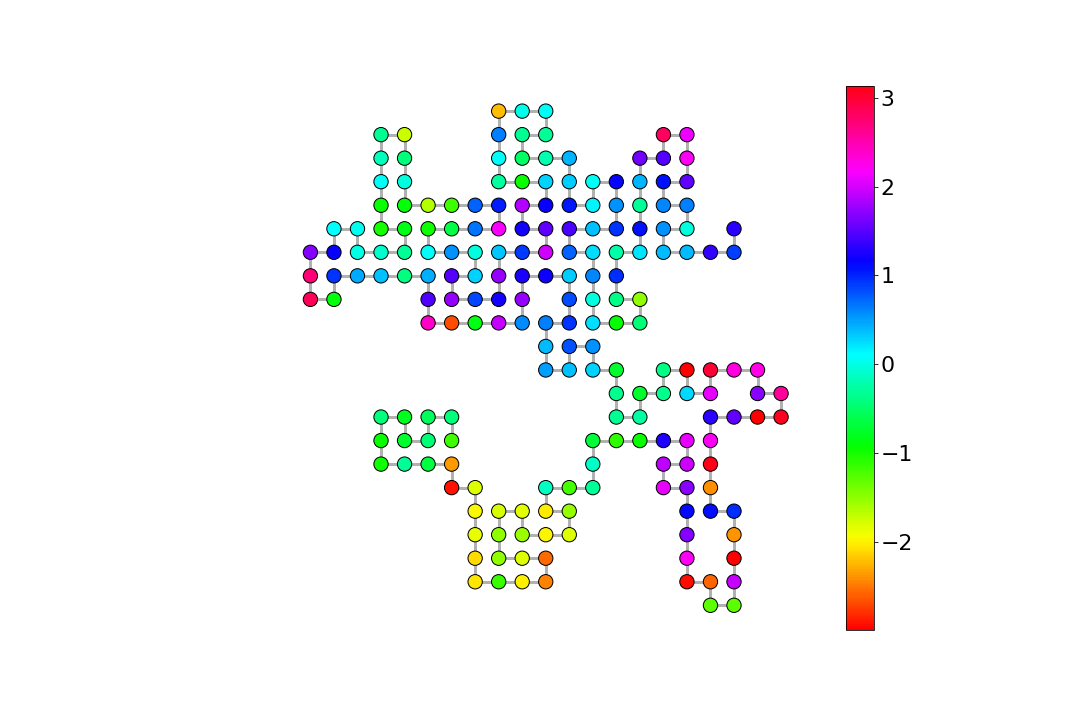
\includegraphics[scale=0.13]{state_example.png} 
	%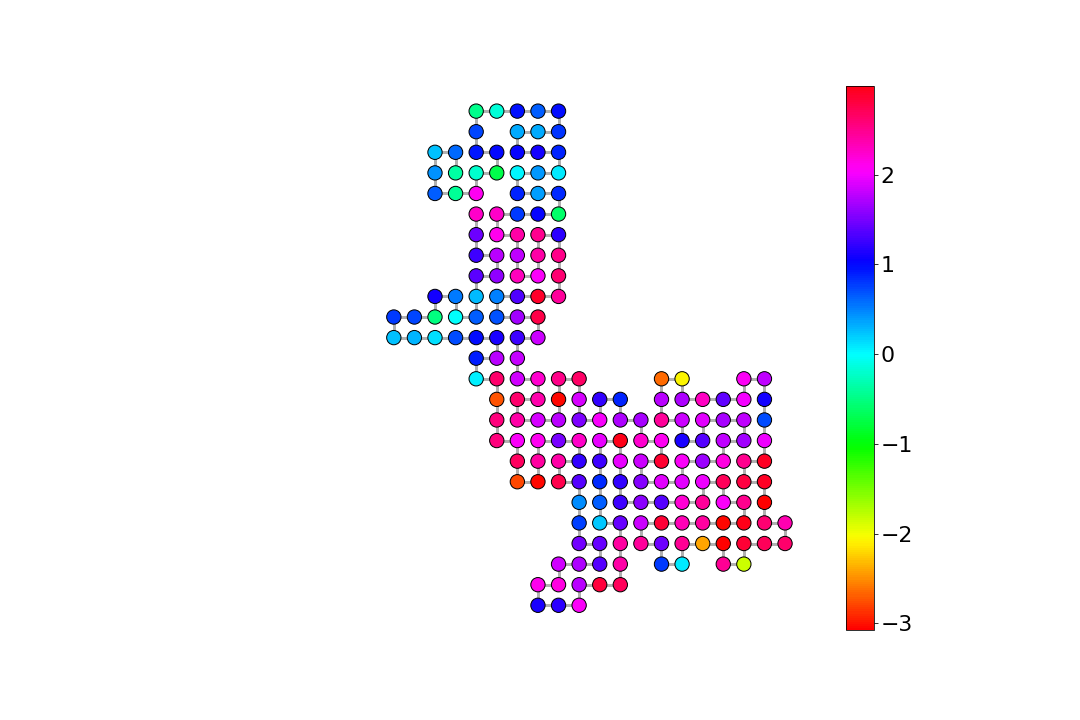
\includegraphics[scale=0.13]{state_example1.png}
			\label{fig:example}
		\end{figure}
		
	\end{multicols}

 Partition function:
\begin{equation*}
\label{partitionfunction}
Z(J) =  \sum_{u \in U_N }  \int_{-\pi}^{\pi}   \frac{1}{ (2 \pi  )^N}
d \theta_1 d \theta_2 \dots d\theta_N
e ^{J \cos(\theta_1-\theta_2)} e ^{J \cos(\theta_2-\theta_3)} \dots 
e ^{J \cos(\theta_{N-1}-\theta_N)} %= 2 \pi
%\prod_{j=2}^{N}  \int_{-\pi}^{\pi} d \theta_j^{'} e ^{J(cos\theta_j^{'})} 
\end{equation*} 
\end{frame}



\begin{frame} 
	\frametitle{Markov chain Monte-Carlo}
	\begin{minipage}{0.44\linewidth}
		\begin{itemize} 
			
			\item  Snake-like algorithm 
			
			 \bigbreak  
			 \bigbreak  
			 \bigbreak  
			 \bigbreak  
			
			\item Reconnect
			
			\bigbreak  
			\bigbreak  
			\bigbreak  
			\bigbreak  
			 
			\item Wolff cluster update 
			\bigbreak  
			\bigbreak  
			\bigbreak  
			
		\end{itemize} 
		
	\end{minipage}%
	\hfill
	\begin{minipage}{0.56\linewidth}
		%\centering
		\begin{figure}[h]
			\centering
			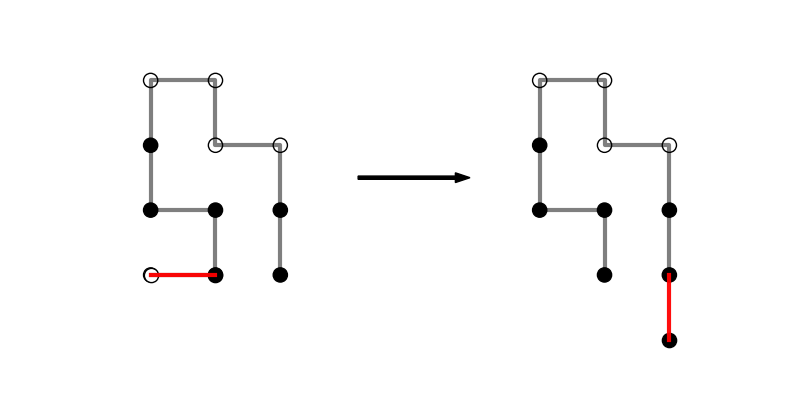
\includegraphics[scale=0.22]{snakeupdate.png} \\
			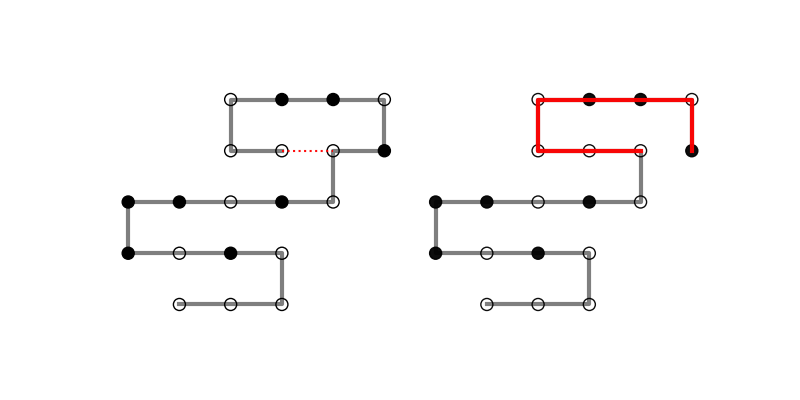
\includegraphics[scale=0.22]{reconnect.png} \\ 
			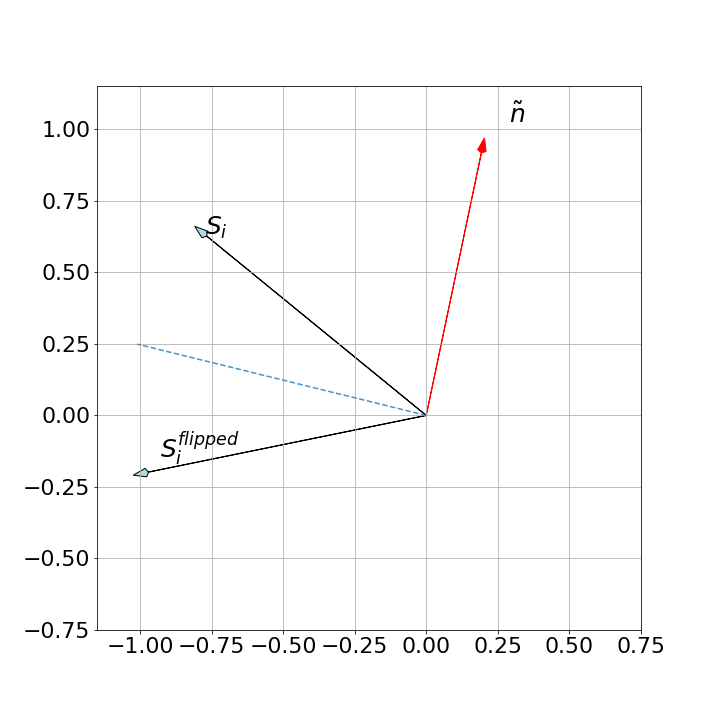
\includegraphics[scale=0.122]{cluster_flip.png}
			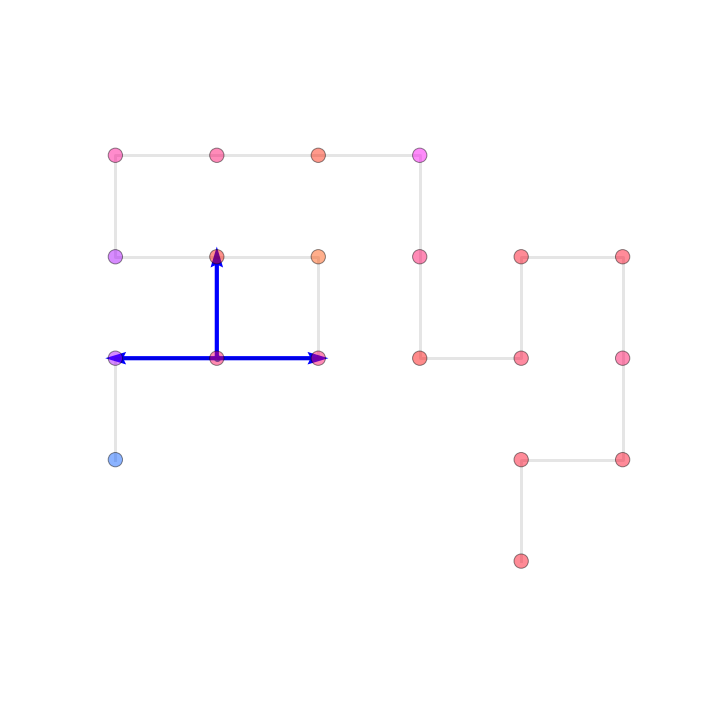
\includegraphics[scale=0.122]{state_example_cluster.png}
			%\scriptsize {\par { \tiny{  $\approx 5 \times 10^{11}$ итераций }} } 
			\label{ph}
		\end{figure}
	\end{minipage}
\end{frame}



\section{Phase transition, 2D }
\subsection{Structural transtition }

\begin{frame} 
	\frametitle{\insertsection}
	\framesubtitle{\insertsubsection}
	\begin{minipage}{0.48\linewidth}
		\begin{itemize} 
			
			\item $ \langle R_N^2 \rangle_x \sim N^{2 \nu(x)}  $
			\item iSAW: $\nu_{\theta} = \frac{4}{7}$
	   \begin{equation*}
	 \label{berettiscale}
	 \log (R_N^2+k_1 ) = 2 \nu \log (N+k_2) + b
	 \end{equation*}
	 
	 		\begin{figure}[h]
	 	\centering
	 	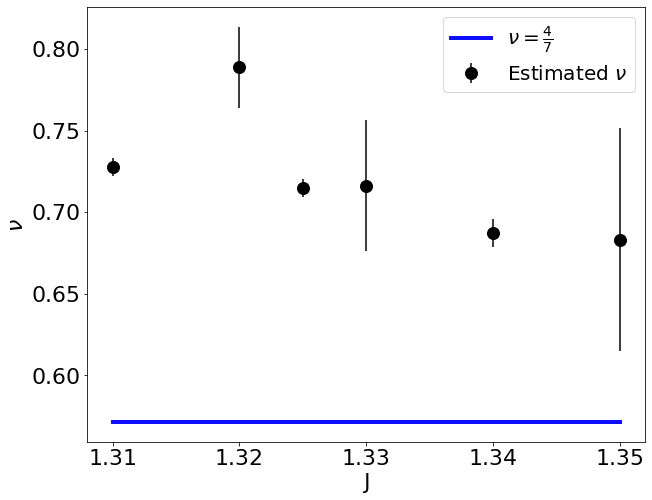
\includegraphics[scale=0.1822]{nu_shortchains_1.png} 
	 	%\scriptsize {\par { \tiny{  $\approx 5 \times 10^{11}$ итераций }} } 
	 
	 \end{figure}
		\end{itemize} 
		
	\end{minipage}%
	\hfill
	\begin{minipage}{0.48\linewidth}
		%\centering
		\begin{figure}[h]
			\centering
			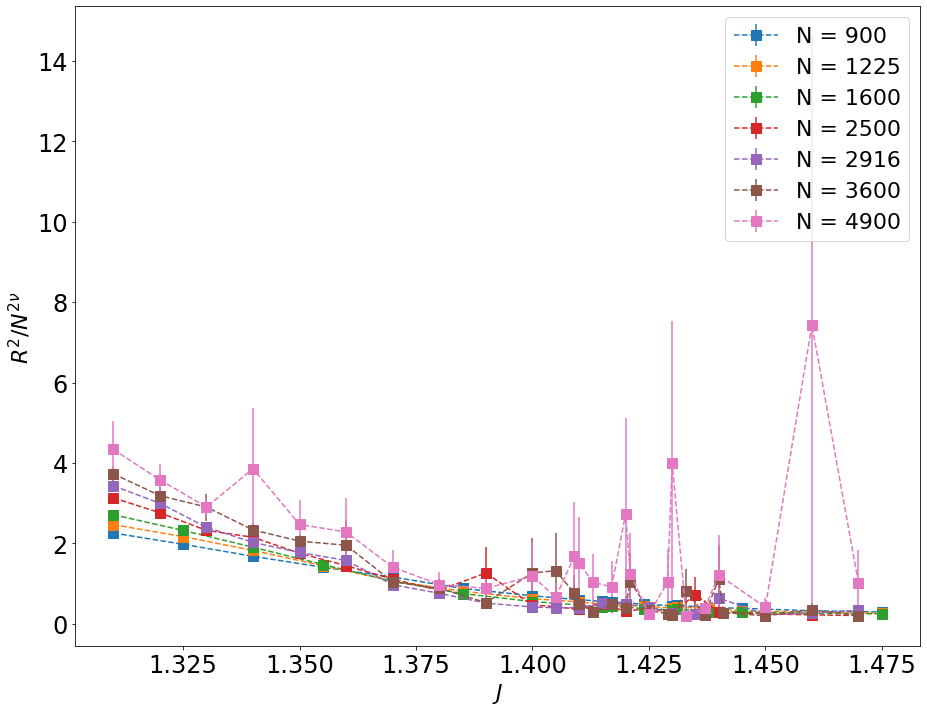
\includegraphics[scale=0.1822]{rscaling_longchains.png} 
			%\scriptsize {\par { \tiny{  $\approx 5 \times 10^{11}$ итераций }} } 
			\label{ph}
		\end{figure}
	\end{minipage}
\end{frame}


\section{Phase transition, 2D }
\subsection{Magnetic transtition }

\begin{frame} 
	\frametitle{\insertsection}
	\framesubtitle{\insertsubsection}
	\begin{minipage}{0.48\linewidth}
		\begin{itemize} 
			
			\item The mean magnetization :
			\Scale[0.75]{
			\langle \vec{m} \rangle = \frac{1}{N} \left\langle ( \sum_{i=1}^{N} cos \theta_i, \sum_{i=1}^{N} sin \theta_i  ) \right\rangle}
 
			
		\item 	The second moment:
		\Scale[0.75]{
			\langle m^2 \rangle = \frac{1}{N^2} \left\langle ( \sum_{i=1}^{N} cos \theta_i )^2 +  (\sum_{i=1}^{N} sin \theta_i  )^2 \right\rangle
			}
		 
		 
       \begin{figure}[h]
		 	\centering
		 	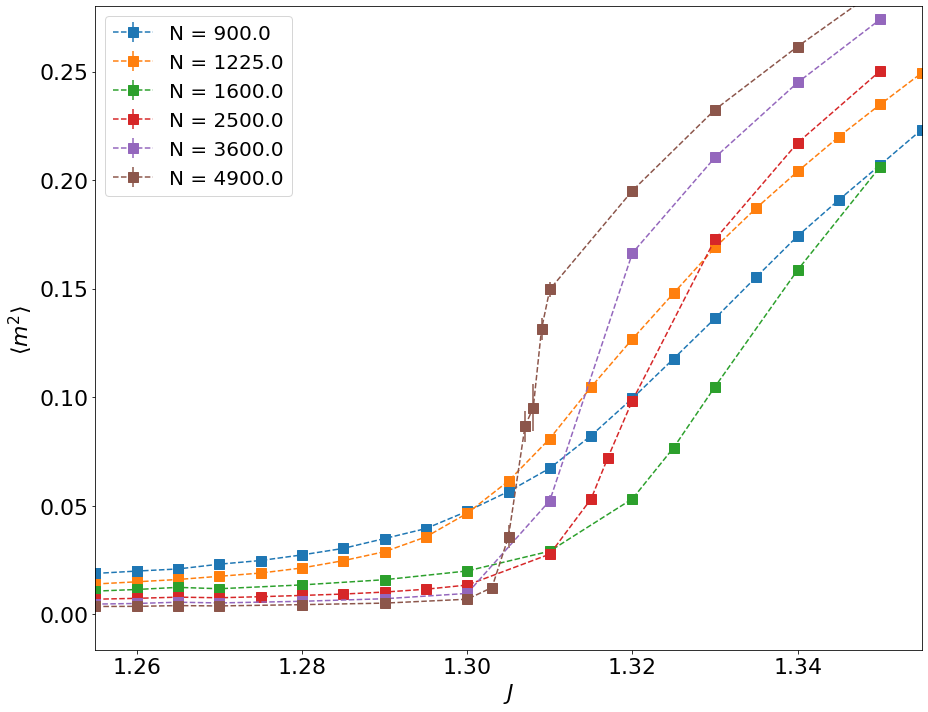
\includegraphics[scale=0.1422]{magnetization2_longchains.png} 
		 	%\scriptsize {\par { \tiny{  $\approx 5 \times 10^{11}$ итераций }} } 
		 	
		 \end{figure}
	 \end{itemize} 
		 
	 
		
	\end{minipage}%
	\hfill
	\begin{minipage}{0.48\linewidth}
		%\centering
		\ \begin{equation*}
		\label{binderqum}
		U_4 (J) = 1 - \frac{ \langle m^4 \rangle}{3 \langle m^2 \rangle^2  }
		\end{equation*}
		\begin{figure}[h]
			\centering
			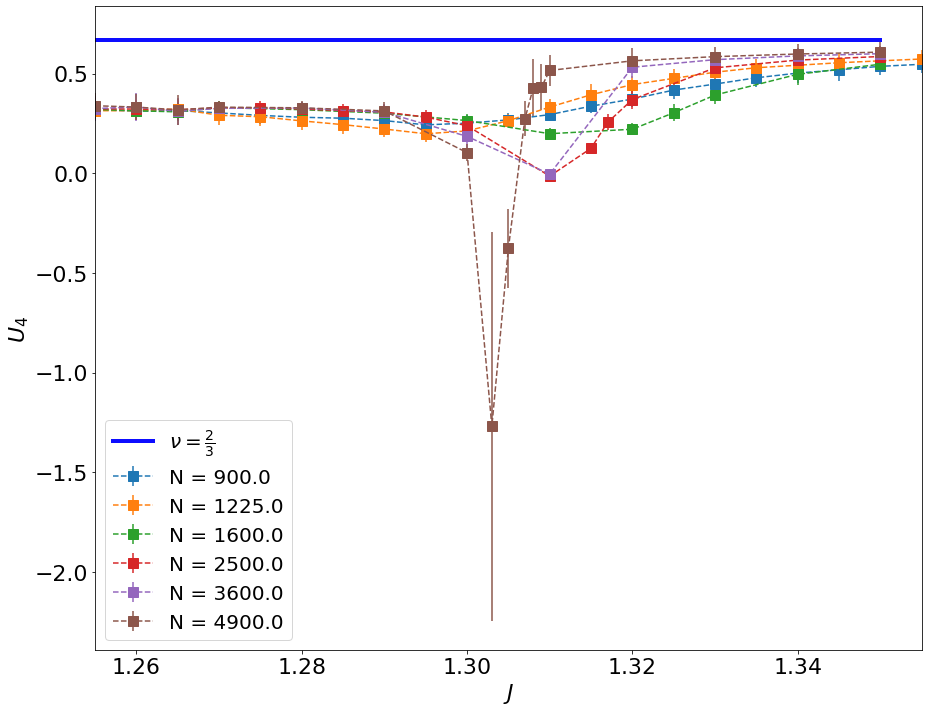
\includegraphics[scale=0.2022]{bindercumulants_longchains.png} 
			%\scriptsize {\par { \tiny{  $\approx 5 \times 10^{11}$ итераций }} } 
			\label{ph}
		\end{figure}
	\end{minipage}
\end{frame}




\begin{frame}
	\frametitle{Transition, 2D}
	\begin{multicols}{2}	
		\begin{figure}[h]
	\centering
	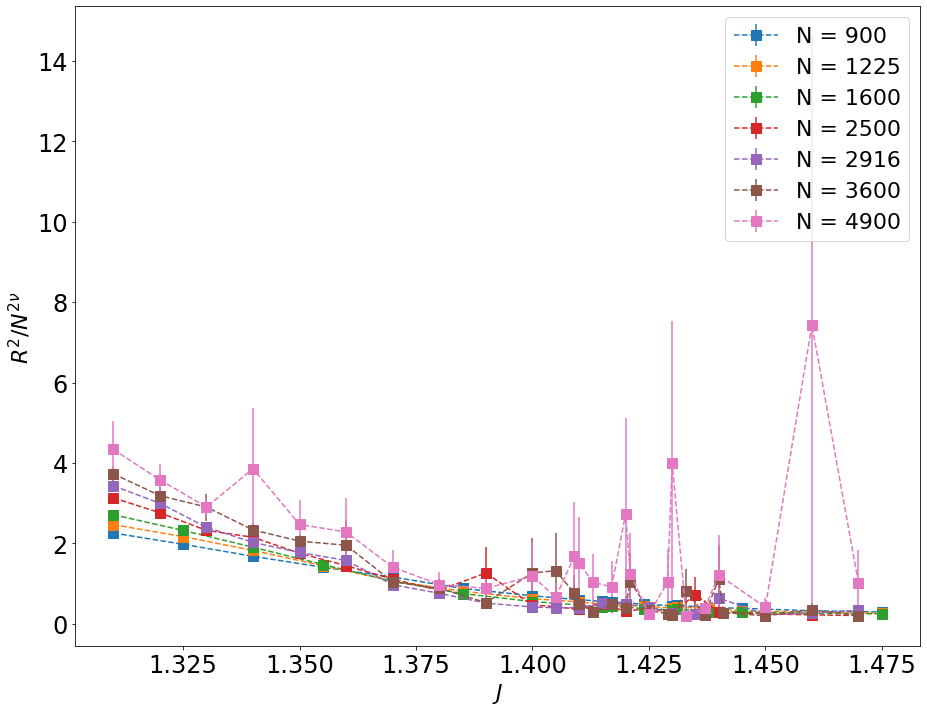
\includegraphics[scale=0.1822]{rscaling_longchains.png} 
	%\scriptsize {\par { \tiny{  $\approx 5 \times 10^{11}$ итераций }} } 
	\label{ph}
\end{figure}
\begin{equation*}
\label{eq:critical_J_theta_2D}
J_{\theta}^{3600} \approx  1.36(1) 
\end{equation*}		
		\columnbreak		
		\begin{figure}[h]
		\centering
		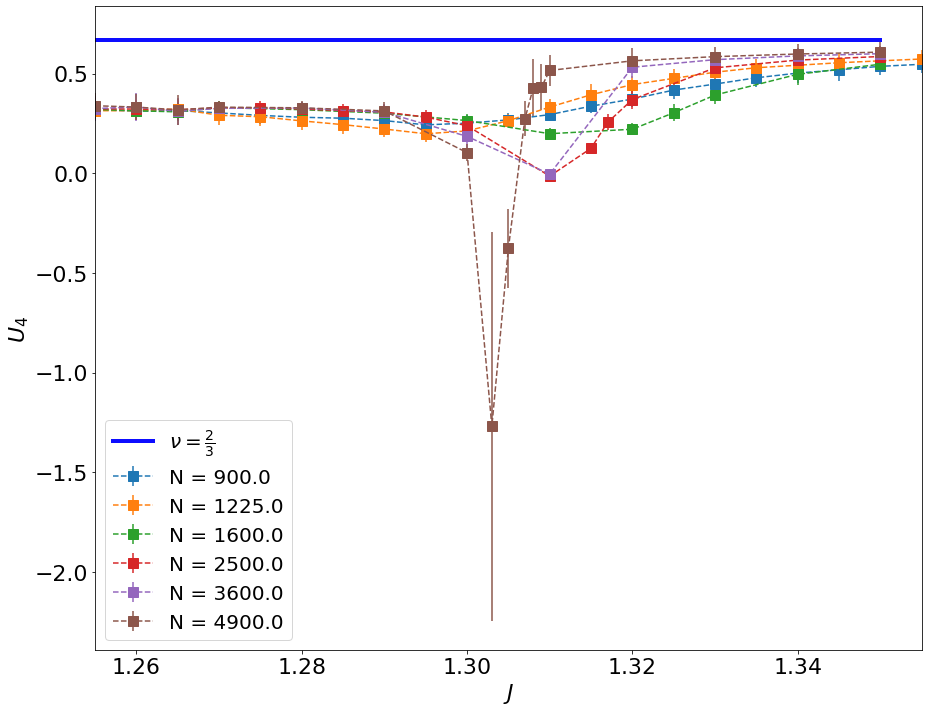
\includegraphics[scale=0.1822 ]{bindercumulants_longchains.png} 
		%\scriptsize {\par { \tiny{  $\approx 5 \times 10^{11}$ итераций }} } 
		\label{ph}
		\end{figure}
		\begin{equation*}
		\label{eq:critical_J_magnet_2D}
		J_{cr}^{3600} \approx  1.43(1)
		\end{equation*}
	\end{multicols}
\end{frame}

\section{Transition, 2D}
\subsection{Distributions }
\begin{frame}
		\frametitle{\insertsection}
	\framesubtitle{\insertsubsection}
   \begin{figure}
 	\centering
 	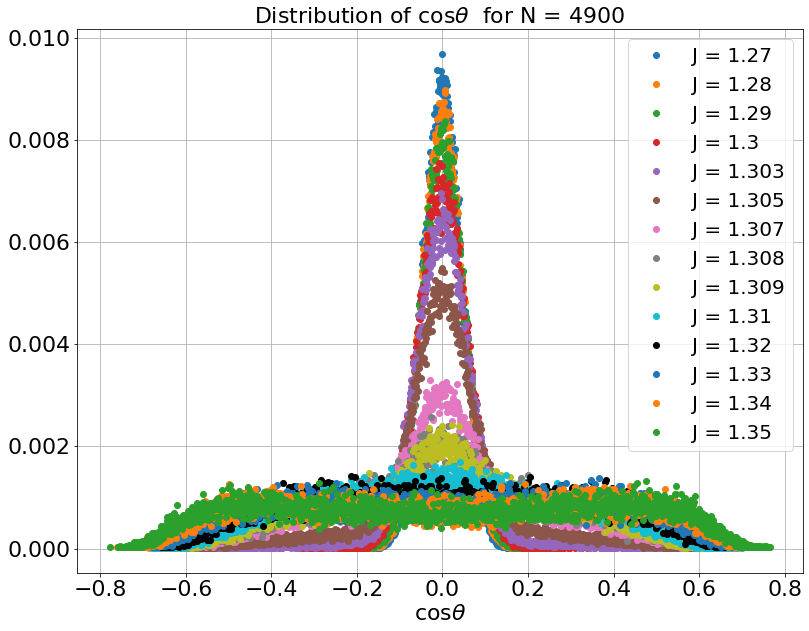
\includegraphics[scale=0.1825]{Images/distr_cos_4900.png}
 	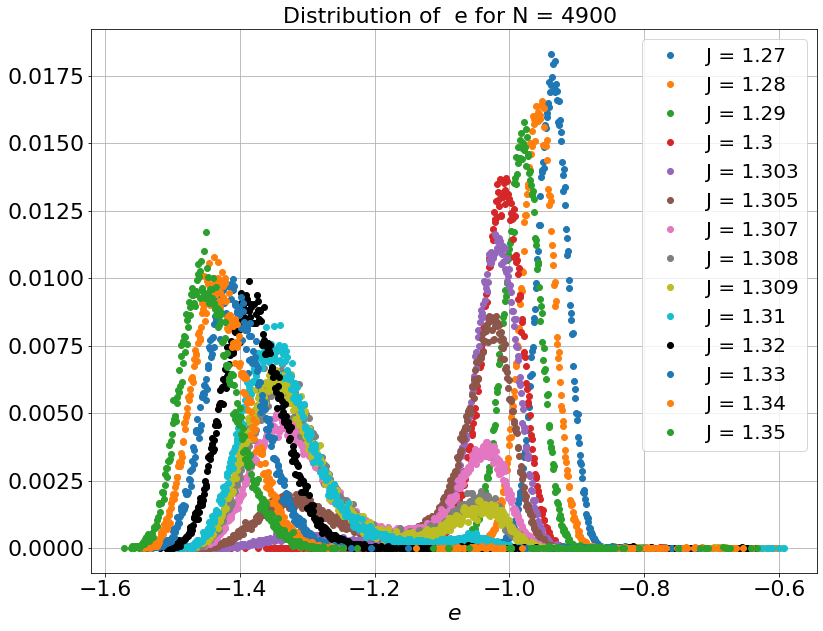
\includegraphics[scale=0.1825]{Images/distr_energy_4900.png}
 	%\caption{ Distributions for chains $N=2500$ and $N=4900$ for various $J$.    }
 	\label{fig:distributions}
 \end{figure}
 \centering	No bimodal energy, no signs of first-order transition 
\end{frame}

\section{Phase transition, 3D }
\subsection{Structural transtition }

\begin{frame} 
	\frametitle{\insertsection}
	\framesubtitle{\insertsubsection}
	\begin{minipage}{0.48\linewidth}
		\begin{itemize} 
			
			\item $ \langle R_N^2 \rangle_x \sim N^{2 \nu(x)}  $
			\item iSAW: $\nu_{\theta} = \frac{1}{2}$
			\begin{equation*}
			\label{berettiscale}
			\log (R_N^2+k_1 ) = 2 \nu \log (N+k_2) + b
			\end{equation*}
			
			\begin{figure}[h]
				\centering
				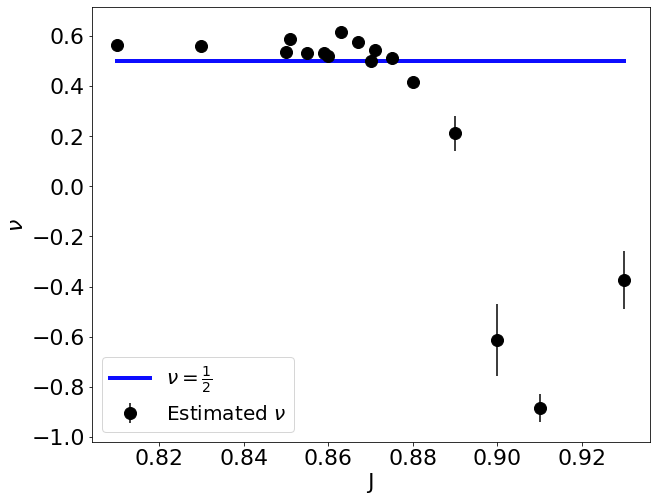
\includegraphics[scale=0.1822]{3_nu_shortchains_deep.png} 
				%\scriptsize {\par { \tiny{  $\approx 5 \times 10^{11}$ итераций }} } 
				
			\end{figure}
		\end{itemize} 
		
	\end{minipage}%
	\hfill
	\begin{minipage}{0.48\linewidth}
		%\centering
		\begin{figure}[h]
			\centering
			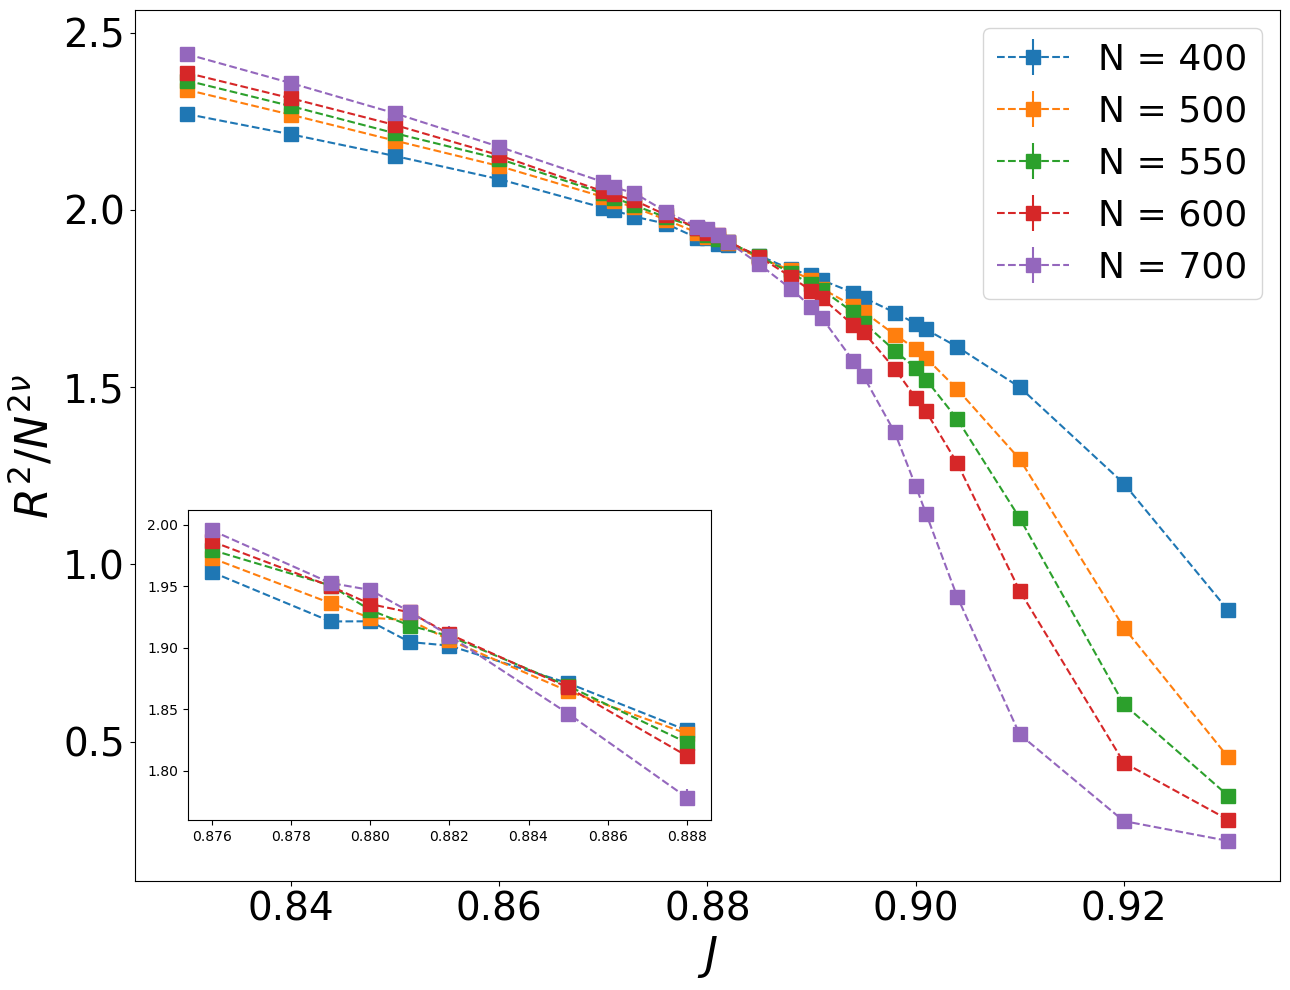
\includegraphics[scale=0.1822]{3_rscaling_longchains.png} 
			%\scriptsize {\par { \tiny{  $\approx 5 \times 10^{11}$ итераций }} } 
			\label{ph}
		\end{figure}
	\end{minipage}
\end{frame}


\begin{frame}
	\frametitle{Transition, 3D}
	\begin{multicols}{2}	
		\begin{figure}[h]
			\centering
			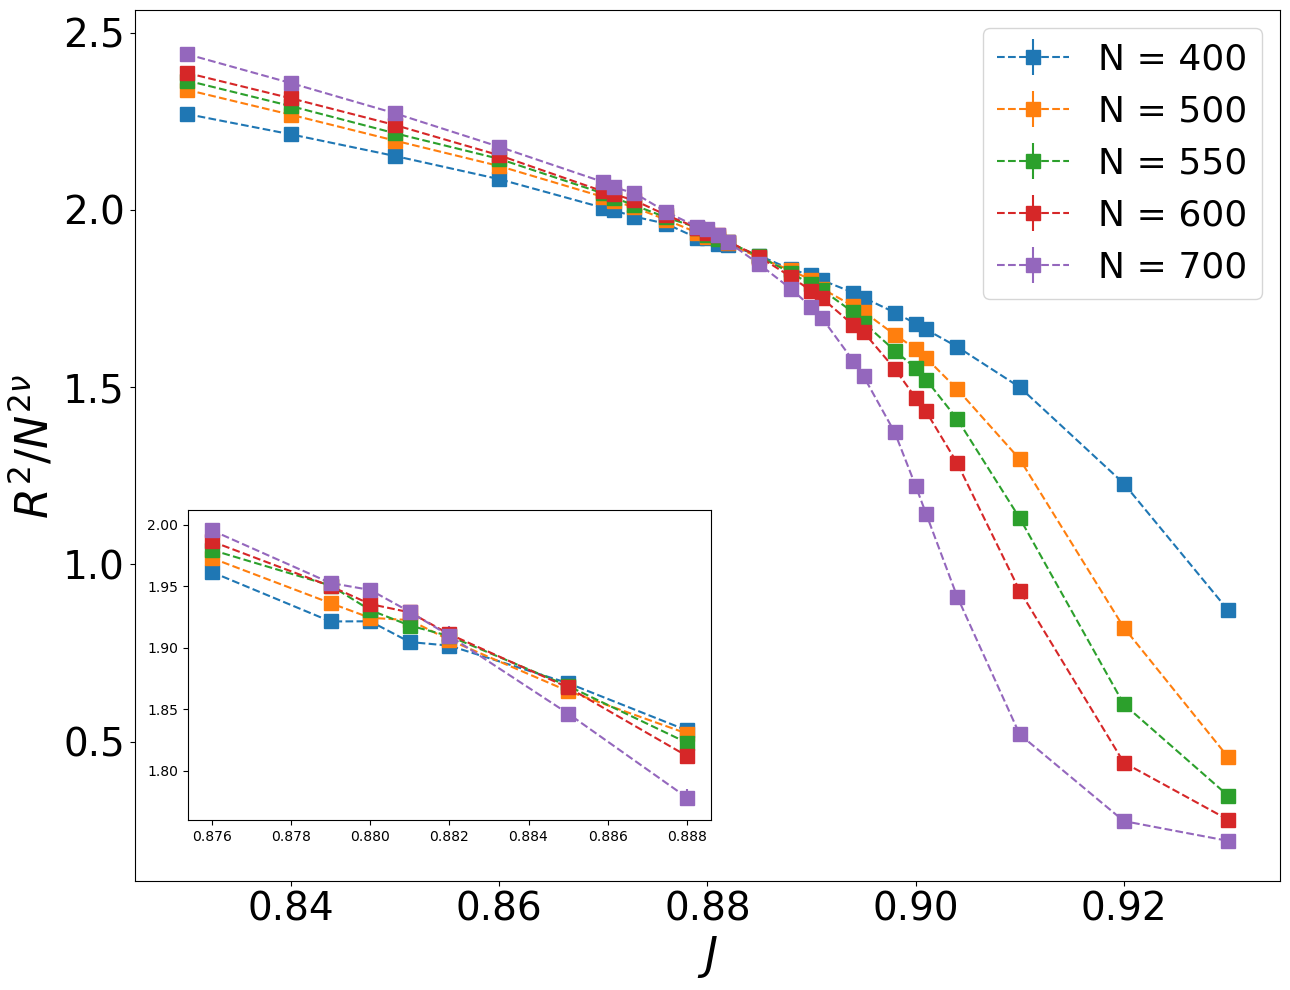
\includegraphics[scale=0.1822]{3_rscaling_longchains.png} 
			%\scriptsize {\par { \tiny{  $\approx 5 \times 10^{11}$ итераций }} } 
			\label{ph}
		\end{figure}
		\begin{equation*}
		\label{eq:critical_J_theta_2D}
		J_{\theta}^{700} \approx 0.876(5)     
		\end{equation*}		
		\columnbreak		
		\begin{figure}[h]
			\centering
			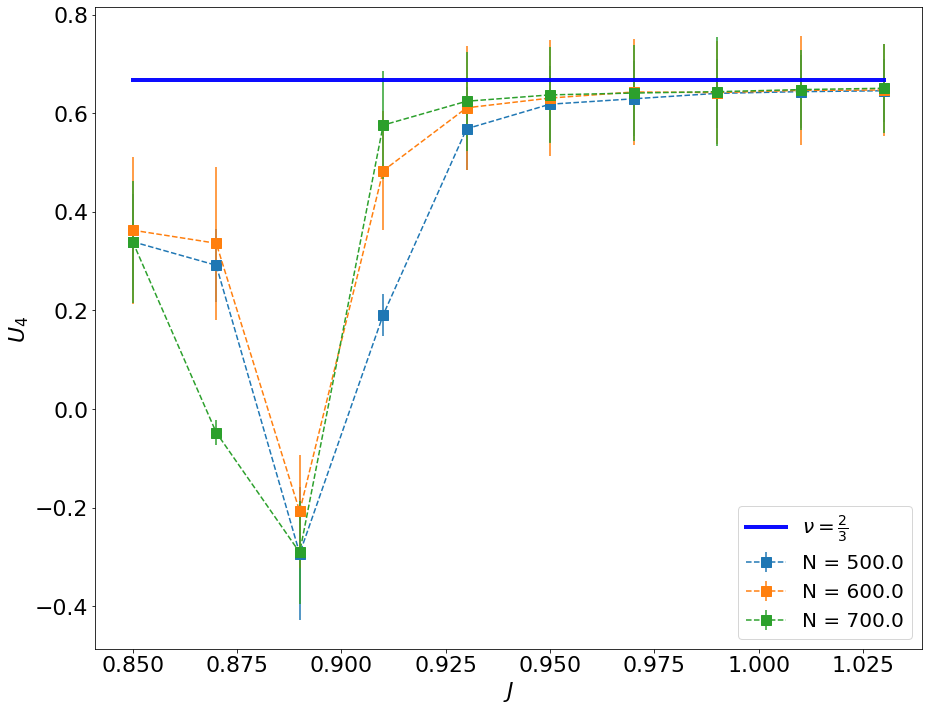
\includegraphics[scale=0.1822 ]{3_bindercumulants_longchains.png} 
			%\scriptsize {\par { \tiny{  $\approx 5 \times 10^{11}$ итераций }} } 
			\label{ph}
		\end{figure}
	\end{multicols}
\end{frame}


\section{Transition, 3D}
\subsection{Distributions }
\begin{frame}
	\frametitle{\insertsection}
	\framesubtitle{\insertsubsection}
	\begin{figure}
		\centering
		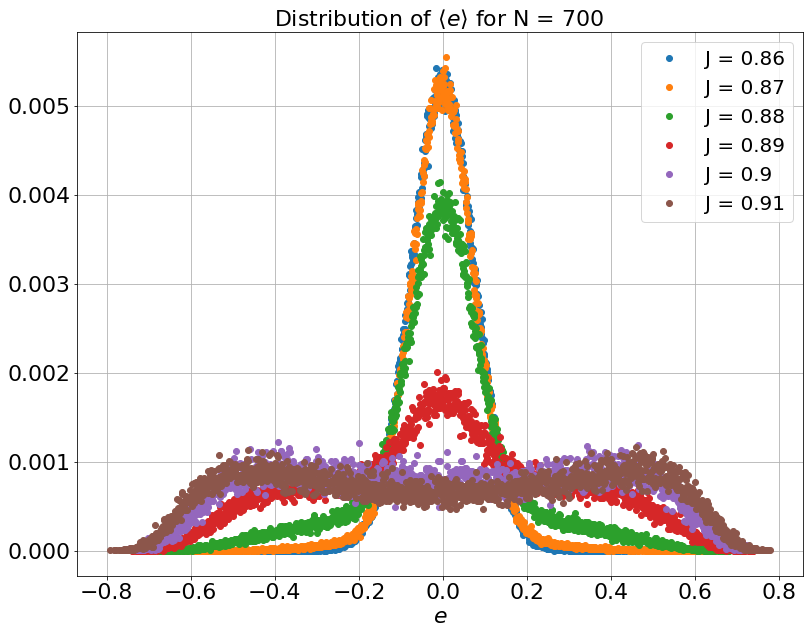
\includegraphics[scale=0.1825]{Images/distr_cos_700.png}
		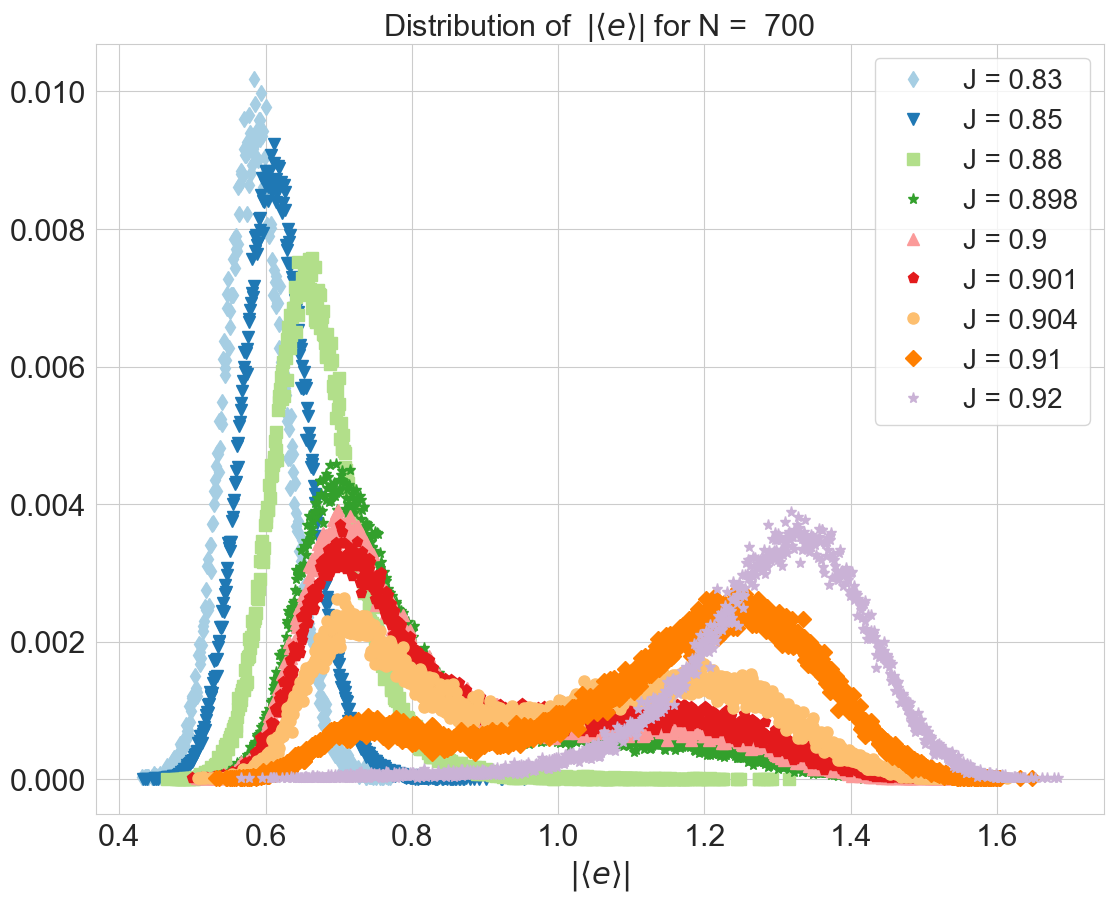
\includegraphics[scale=0.1825]{Images/distr_energy_700.png}
		%\caption{ Distributions for chains $N=2500$ and $N=4900$ for various $J$.    }
		\label{fig:distributions}
	\end{figure}
	
	 \centering	Bimodal energy, signs of first-order transition 
	
\end{frame}


\section{Conclusions and outlook}
\begin{frame}
	\frametitle{\insertsection}
	\framesubtitle{\insertsubsection}
	\begin{itemize}
		\item For 3D case, MC data indicates first-order transition 
		\item  For 2D case, MC data is inconclusive, whether the transitions occur simultaneously or at distinct values of the coupling constant J. More work is needed to conclusively rule out one of possibilities. 
		 
	\end{itemize}
	\begin{figure}[b]
		\centering
		%\includegraphics[scale=0.25]{question} 
		\scriptsize {\par { \scriptsize{    }} } 
		\label{ph}
	\end{figure}
	
\end{frame}


\end{document}